\documentclass[prb,12pt]{revtex4-2}

\usepackage{amsmath, amssymb,physics,amsfonts,amsthm}
\usepackage[most]{tcolorbox}
\usepackage{enumitem}
\usepackage{cancel}
\usepackage{booktabs}
\usepackage{polynom}
\usepackage{tikz}
\usepackage{hyperref}
\usepackage{enumitem}
\usepackage{transparent}
\usepackage{float}
\usepackage{multirow}
\newtheorem{Theorem}{Theorem}
\newtheorem{Proposition}{Theorem}
\newtheorem{Lemma}[Theorem]{Lemma}
\newtheorem{Corollary}[Theorem]{Corollary}
\newtheorem{Example}[Theorem]{Example}
\newtheorem{Remark}[Theorem]{Remark}
\theoremstyle{definition}
\newtheorem{Problem}{Problem}
\theoremstyle{definition}
\newtheorem{Definition}[Theorem]{Definition}
\newenvironment{parts}{\begin{enumerate}[label=(\alph*)]}{\end{enumerate}}
%tikz
\usetikzlibrary{patterns}
\usetikzlibrary{matrix}
%tcolorbox
\tcbset{breakable=true,toprule at break = 0mm,bottomrule at break = 0mm}
% definitions of number sets
\newcommand{\N}{\mathbb{N}}
\newcommand{\R}{\mathbb{R}}
\newcommand{\Z}{\mathbb{Z}}
\newcommand{\Q}{\mathbb{Q}}
\newcommand{\C}{\mathbb{C}}
\allowdisplaybreaks
\begin{document}
\title{Fortgeschrittene Fehlerrechnung Übungsblatt 1}
	\author{Jun Wei Tan}
	\email{jun-wei.tan@stud-mail.uni-wuerzburg.de}
	\affiliation{Julius-Maximilians-Universit\"{a}t W\"{u}rzburg}
	\date{\today}
	\maketitle

\section{Grund der Annahme}
\begin{tcolorbox}
	Weshalb könnte man mit den gegebenen Informationen davon ausgehen, dass die registrierten $\gamma$-Quanten einer Poissonverteilung folgen?
\end{tcolorbox}
Die Population ist unendlich. Die maximale Anzahl von Ereignisse ($n$) ist groß, da wir 10 g haben und ein Molekül leicht ist. Allerdings ist $n\cdot p$ wahrscheinlich sehr klein, da die Halbwertzeit $>10$ Jahre ist. Die Wahrscheinlichkeit, dass ein Molekül ein $\gamma$-Quanten emittiert, ist $1-e^{\frac{(1\text{s})\ln 2}{t_{1/2}}}$, also sehr klein. Insgesamt ist die beste Verteilung eine Poissonverteilung.
\section{Datentabelle}
\begin{align*}
	\text{Mittelwert}:&~\mu=2,73214\\
	\text{Standardabweichung}:&~\sigma=1,67784\\
	\text{Anzahl der Messungen}:&~n=336\\
	\text{Standardfehler}:&~s=\frac{\sigma}{\sqrt{n}}\approx 0,0050
\end{align*}
Insgesamt ist
\[\mu=(2,7321\pm 0,0050)\]
\begin{table}[h]
	{\scriptsize
\begin{tabular}{cccccccccc}
	\toprule
	\textbf{Ereignisse} & 0 & 1 & 2 & 3 & 4 & 5 & 6 & 7 & 8 \\\midrule
	H\"{a}ufigkeit & 11 & 89 & 65 & 71 & 48 & 28 & 16 & 6 & 2 \\\midrule
	Relative H\"{a}ufigkeit & 0,032738 & 0,26488 & 0,19345 & 0,21131 & 0,14286 & 0,083333 & 0,047619 & 0,017857 & 0,0059524 \\\midrule
	Poisson-Wahrscheinlichkeit & 0,0650797 & 0,177807 & 0,242897 & 0,22121 & 0,151094 & 0,0825622 & 0,0375953 & 0,0146737 & 0,00501132 \\\bottomrule
\end{tabular}
}
\end{table}

\section{Histogramm}
\begin{figure}[h]
	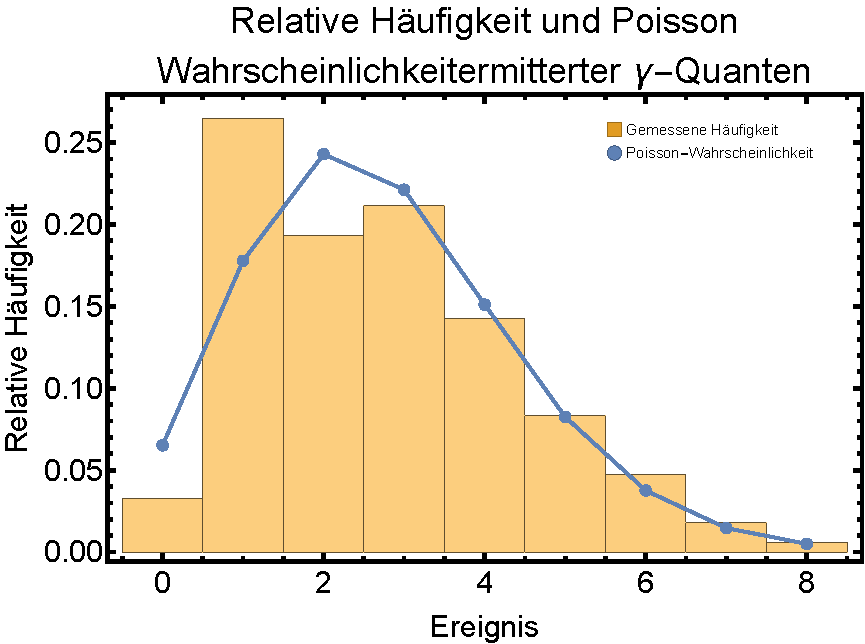
\includegraphics[width=0.6\textwidth]{fig1.pdf}
	\caption{Jun Wei Tan 25.04.24}
\end{figure}

\section{Zentrale $\chi^2$ Verteilung}
Dichtefunktion:
\[f_{\chi^2_n}=\frac{1}{2^{\frac n2}\left(\frac n2-1\right)!}x^{\frac n2 - 1}\exp\left(-\frac x2\right)\]
Erwartungswert

\begin{align*}
	E[x]=& \int_{\text{Supp }f}f_{\chi_n^2}(x) x\dd{x}\\
	=&\int_0^\infty \frac{1}{2^{\frac n2}\left( \frac{n}{2}-1 \right)! }x^{\frac{n}{2}-1}\exp\left( -\frac{x}{2} \right) x\dd{x}\\
	=&\frac{1}{2^{\frac{n}{2}}\left( \frac{n}{2}-1 \right)! }\int_0^\infty x^{\frac{n}{2}}\exp\left( -\frac{x}{2} \right) \dd{x}\\
	=&\frac{2}{2^{\frac{n}{2}}\left( \frac{n}{2}-1 \right)! }\int_0^\infty (2x)^{\frac{n}{2}}\exp\left( -x \right) \dd{x}\\
	=&\frac{2}{\left( \frac{n}{2}-1 \right)! }\int_0^\infty x^{\frac{n}{2}}\exp\left( -x \right) \dd{x}\\
	=&\frac{2}{\left(\frac{n}{2}-1\right)!}\Gamma\left( \frac{n}{2}+1 \right) \\
	=&\frac{2}{\left( \frac{n}{2}-1 \right)!}\left( \frac{n}{2} \right)!\\
	=& 2(n / 2) = n
\end{align*}
Varianz
\begin{align*}
	\sigma^2=& E[(x-\mu)^2]\\
	=&E[(x-n)^2]\\
	=&\frac{1}{2^{\frac{n}{2}}\left( \frac{n}{2}-1 \right)! }\int_0^\infty x^{\frac{n}{2}-1}\exp\left( -\frac{x}{2} \right) (x-n)^2\dd{x}\\
	=&\frac{1}{2^{\frac{n}{2}}\left( \frac{n}{2}-1 \right)!}\int_0^\infty x^{\frac{n}{2}+1}\exp\left( -\frac{x}{2}\right) \\
	&-2nx^{\frac{n}{2}}\exp\left( -\frac{x}{2} \right) +n^2 x^{\frac{n}{2}-1}\exp\left( -\frac{x}{2} \right) \dd{x}\\
	=& \frac{1}{2^{\frac{n}{2}}\left( \frac{n}{2}-1 \right)! }\left[2^{\frac{n}{2}+2}\Gamma\left( 2+\frac{n}{2} \right) -2^{\frac{n}{2}+1}n^2 \Gamma\left( \frac{n}{2} \right) +2^{\frac{n}{2}}n^2\Gamma\left( \frac{n}{2} \right) \right]\\
	=& \frac{1}{2^{\frac{n}{2}}\left( \frac{n}{2}-1 \right)! }\left[2^{\frac{n}{2}+2}\Gamma\left( 2+\frac{n}{2} \right) -2^{\frac{n}{2}}n^2 \Gamma\left( \frac{n}{2} \right)\right]\\
	=&\frac{4}{\left( \frac{n}{2}-1 \right)!} \left[ \left( \frac{n}{2}+1 \right)! - \left( \frac{n}{2} \right)^2 \left( \frac{n}{2}-1 \right)! \right]\\
	=&4\left[ \left( \frac{n}{2}+1 \right) \frac{n}{2}-\left( \frac{n}{2} \right)^2 \right]\\
	=&2n
\end{align*}
\end{document}
